\newpage
\section{Конструкторская часть}

\newpage
\subsection{Разработка функциональной схемы платы управления}

\newpage
\subsection{Разработка принципиальной схемы платы управления}

\newpage
\subsection{Разработка экспериментального стенда}
\subfile{src/construction/stand_requirements}

\begin{figure}[ht!]
    \centering
    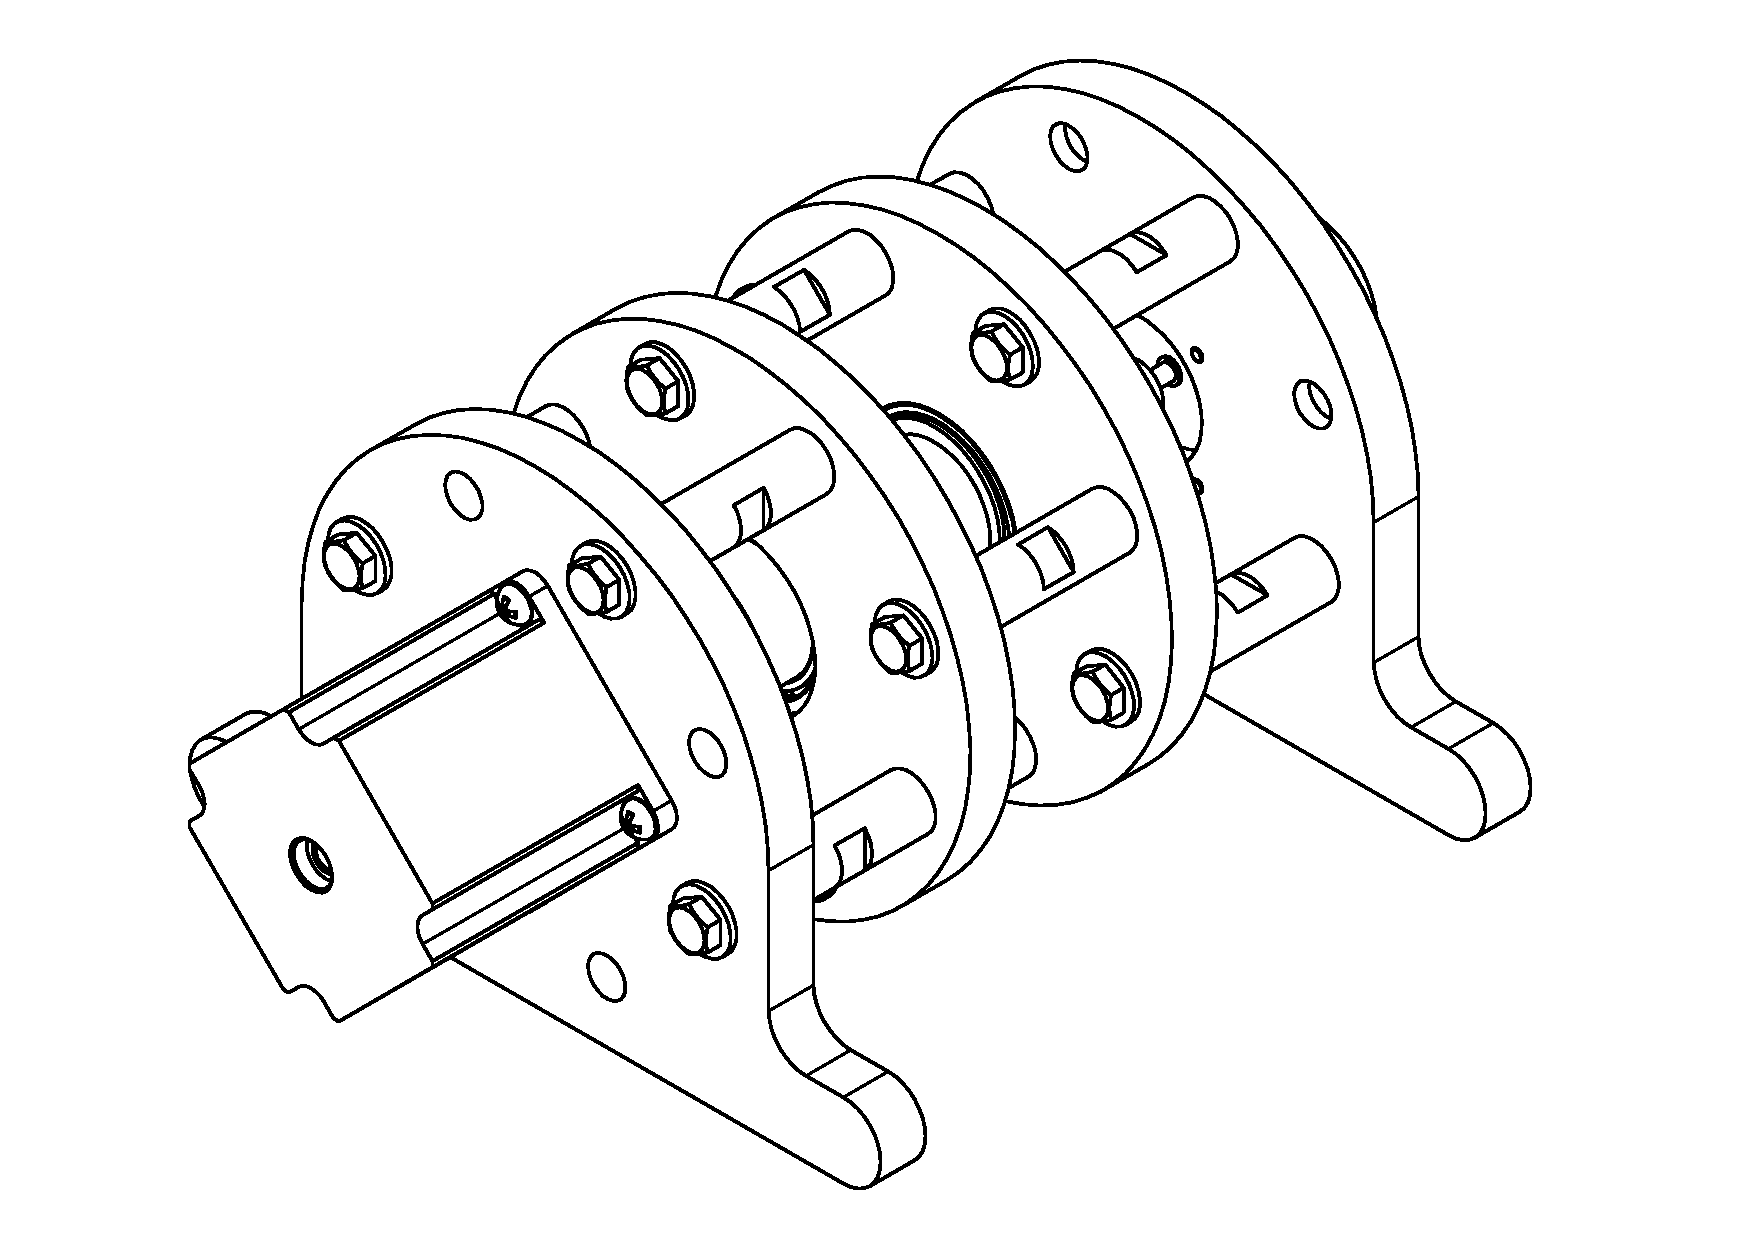
\includegraphics[width=\textwidth, scale=0.6, keepaspectratio]
                    {./src/pictures/stand}
    \caption{Изометрическая проекция экспериментального стенда}
    \label{pic_stand}
\end{figure}

Спроектирован и произведён стенд (рис. \ref{pic_stand}), удовлетворяющий
вышеизложенным требованиям. Стенд предназначен для установки одного датчика угла
и одного двигателя, облатает подшипниковым узлом для избежания чрезмерного
нагружения валов двигателя и датчика. Так же предусмотрена возможность
варьирования момента инерции нагрузки в небольших пределах.

\newpage
\subsection{Разработка программного обеспечения платы управления}
\subfile{src/construction/algo/phase_switch}
